\documentclass{neu_handout}
\usepackage{url}
\usepackage{amssymb}
\usepackage{amsmath}
\usepackage{marvosym}
\usepackage{graphicx}
\usepackage[pdftex]{graphicx}
\usepackage{subfigure}
\graphicspath{ {images/} }
\everymath{\displaystyle}

% Professor/Course information
\title{A Bayseian Approach to Fake News}
\author{Emily Dutile, Shubhi Mittal, Linghan Xing}
\date{December 2017}
\course{CS5100}{Foundations of AI}

\begin{document}
\section*{1 Introduction and Background}

"Fake news" became an increasingly coined term and was almost non-existent in the general context and media providers prior to October 2016 of the Presidential Election. In late 2016, the top 20 fake news stories on Facebook were reported to outperform the top 20 real news stories, which was determined by the number of comments, reactions, and shares. With websites such as Facebook who provide ad revenue to sites that host news stories, it should be the responsibility of these sites to filter out false information in order to correctly inform and educate our society, especially when it comes to presidential elections.

\begin{figure}[h]
\centering
\subfigure[Signal Media]
{
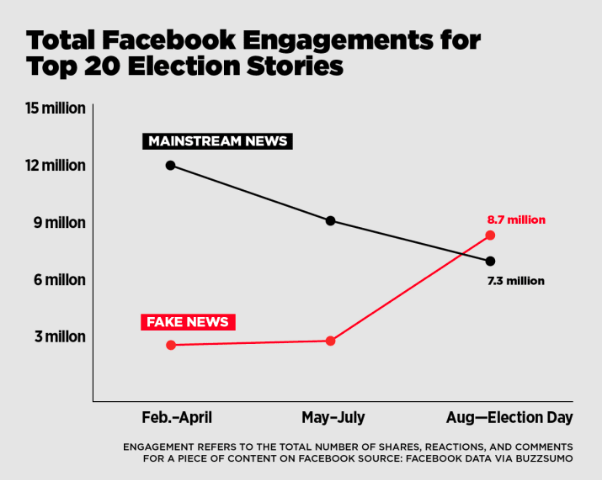
\includegraphics[width=0.3\linewidth]{buzzfeed}
}
\subfigure[BuzzFeed News]
{
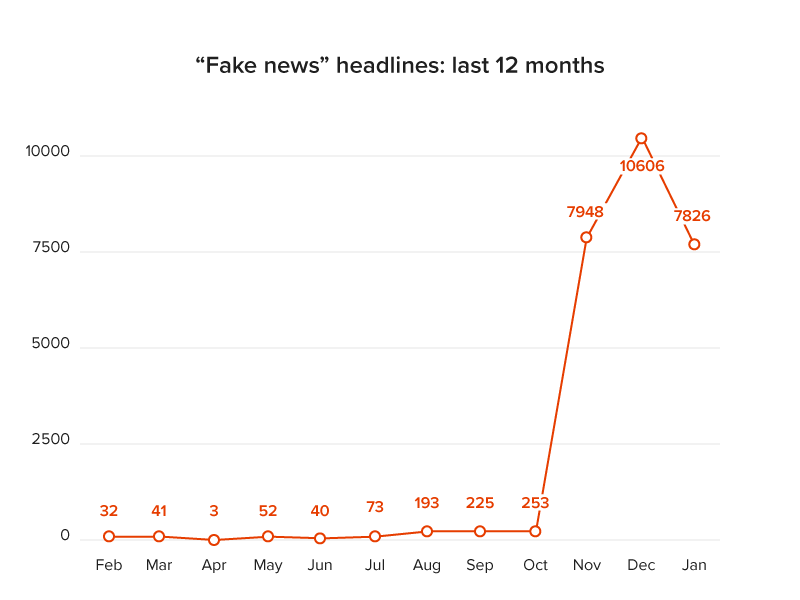
\includegraphics[width=0.3\linewidth]{fakenews}
}
\end{figure}

Fake news posts have exploited the feeds of Facebook users'. Due to this problem, the data science community has looked to respond to this problem through a Kaggle competition called the Fake News Challenge \footnote{http://www.fakenewschallenge.org/}. In our approach to tackle this problem, we have implemented several supervised machine learning based algorithms in order to compare text classifiers on fake news recognition.


\subsection*{1.1 The Data}






\subsection*{1.2 Methods}
We performed supervised machine learning techniques such as naive bayes, multinominal bayes with count vector and TF-IDF, along with SVM and Random Tree Forest. With respect to language processing, tokenization, filtering, lemmatization, and stemming were all used for preprocessing the titles and body text of the articles in the data set. For our evaluation process, we used a confusion matrix to understand the accuracy of our models.

\section*{2. Exploratory Analysis}


\section*{3 Supervised Analysis}
\subsection*{3.1 Naive Bayes}

\subsection*{3.2 Multinominal Naive Bayes}

\subsubsection*{3.2.1 Count Vectorization}


\subsubsection*{3.2.2 TF-IDF}


\subsection*{3.2 SVM}

\subsection*{3.3 Random Forest}
 
 
\subsection*{3.4 Neural Network}


\section*{4 Discussion}


\begin{thebibliography}{9}

\bibitem{ai} 
Russel and Norvig. 
\textit{Artificial Intelligence: A Modern Approach, 3rd Ed.}. 

 
\bibitem{buzzfeed}  
\textit{This Analysis Shows How Viral Fake Election News Stories Outperformed Real News on Facebook}.
[\textit{BuzzFeed News, November 2016}].
\url{https://www.buzzfeed.com/craigsilverman/viral-fake-election-news-outperformed-real-news-on-facebook?utm_term=.tnpJN34BM#.yfV6V10ZX}.
 

\bibitem{Signal}  
\textit{12 Months of Fake News Headlines, Dissected with Media Monitoring}. 
 \url{https://signalmedia.co/media-monitoring-blog/fake-news-dissected-media-monitoring/}.

\end{thebibliography}


\end{document}